\documentclass[algorithm,pgfplots,colortheme=dark]{cuzbeamer}
\usepackage[ngerman]{babel}
\usepackage[scale=2]{ccicons}
\usepackage{listings}
\usepackage{csquotes}

\newcommand{\py}[1]{\mintinline{python}{#1}}
\newcommand{\pybw}[1]{\mintinline[style=bw]{python}{#1}}
\newcommand{\bash}[1]{\mintinline{bash}{#1}}
\newcommand{\spacechar}{\texttt{\char32\hspace{2pt}}}

\begin{document}
\title{Programmieren mit Python}
\subtitle{Eine Einführung}
\date{\today}
\author{Dr. Aaron Kunert}
\email{aaron.kunert@salemkolleg.de}
\maketitle



%\section{Zu Beginn \dots}

\begin{frame}
\begin{block}{Kurze Vorstellungsrunde}
	\vspace{2pt}
	Schaffst Du es \emph{in 60 Sekunden} folgende Fragen möglichst knackig und aussagekräftig zu beantworten?
	\begin{itemize}
		\item Wer bist Du? 
		\item Windows, Mac oder Linux?
		\item Welche Vorkenntnisse hast Du beim Programmieren?  
		\item Warum hast Du Dich zum Python-Kurs angemeldet? 
		\item Wann wäre der Kurs für Dich perfekt gelaufen? (Best Case Szenario)
		\item Wann würdest Du den Kurs nicht weiter besuchen? (Worst Case Szenario)
	\end{itemize}
\end{block}
\end{frame}


\begin{frame}
	\begin{block}{Ablauf des Kurses}
		\begin{itemize}
			\item Mischung aus Vortrag, Live-Coding und Präsenzübungen
			\item Im Idealfall: Mehr Praxis statt Erklärungen
			\item Jede Woche gibt's ein Aufgabenblatt $\rightarrow$ Besprechung in der nächsten Woche
			\item Kommunikation über Slack: \texttt{https://bit.ly/3a5W9fE} 
			%\texttt{python-kurs.slack.com} 
			(freiwillig)
		\end{itemize}
	\end{block}
\end{frame}

\begin{frame}
	\begin{block}{Warum Python?}
		\begin{itemize}
			\item Einfaches Setup
			\item Einstiegsfreundliche Syntax
			\item Python ist eine Hochsprache
			\item Python muss nicht kompiliert, sondern nur interpretiert werden
			\item Große Community $\rightarrow$ großes \emph{Ecosystem}
			\item Python ist extrem vielseitig
			\item Python ist plattformunabhängig
		\end{itemize}
	\end{block}
\end{frame}

\begin{frame}
	\begin{block}{Typische Einsatzbereiche}
		\begin{itemize}
			\item Automatisierung
			\item Webscraping
			\item Datenanalyse
			\item Webentwicklung
		\end{itemize}
	\end{block}
\end{frame}

\begin{frame}
\begin{block}{Phasen des Lernens einer Programmiersprache}
	\vspace{2pt}
	\uncover<+->{
\begin{enumerate}[<+->]
	\item Annäherung:  Fokus auf dem Begreifen der Grundkonzepte
	\item Syntax: Fokus auf der korrekten Anwendung der Syntax
	\item Funktionalität: Fokus liegt darauf, Problemstellungen \emph{pragmatisch} zu lösen
	\item Design: Fokus auf les-und wartbaren Code
	\item Architektur: Fokus auf Strategie, Projekte nachhaltig und erweiterbar umzusetzen 
\end{enumerate}
	}
\end{block}
\end{frame}


\begin{frame}
	\metroset{block=fill}
	\uncover<+->{\begin{block}{Was wird benötigt?}
			\vspace{2pt}
			\uncover<+->{
				\textbf{Am Anfang}
				\begin{itemize}
					\item Compiler/Interpreter
					\item Texteditor (z.B. Mac: Xcode, Windows: Edit)
				\end{itemize}
			}
			\uncover<+->{
				\textbf{Später}
				\begin{itemize}
					\item Google
					\item Integrierte Entwicklungsumgebung (IDE)
					\item Versionskontrolle (VCS)
					\item Virtueller Maschinen
					\item Datenbanken
					\item Grafikbearbeitung
				\end{itemize}
			}
	\end{block}}
\end{frame}

\begin{frame}
\begin{block}{Wo findet man Hilfe/Infos?}
	\vspace{2pt}
	\begin{itemize}
		\item Google
		\item \texttt{stackoverflow.com}
		\item Youtube (z.B. Tutorials)
		\item Austausch über Slack 
		\item \texttt{docs.python.org/3}
		\item Bücher (z.B. \textit{Python Crashkurs} v. \textsc{Eric Matthes})
		\item \texttt{mailto: aaron.kunert@salemkolleg.de}
	\end{itemize}
\end{block}
\end{frame}


\section{Installation von Python}

\begin{frame}
\begin{block}{Ist Python schon installiert ?}
	\begin{itemize}
		\item Öffne ein Terminal/die Eingabeaufforderung
		\item Gib ein \bash{python --version}
		\item oder alternativ \bash{python3 --version}
		\item Erhältst Du die Antwort \bash{Python} und eine Zahl $\geq 3.6$, dann ist alles fein
		\item Falls nicht: Installiere Python!
	\end{itemize}
\end{block}
\end{frame}


\begin{frame}
\begin{block}{Installation}
\begin{enumerate}
	\item Gehe auf https://www.python.org/downloads/
	\item Klicke den Button "Download Python 3.9.3."
	\item Führe die Installationsdatei aus
	\item Falls Du gefragt wirst, bestätige, dass Python zum PATH hinzugefügt wird
	\item Eventuell muss der Rechner neu gestartet werden
\end{enumerate}	
\end{block}

\begin{alertblock}{Achtung bei Windows}
\vspace{2pt}
Python muss zum PATH hinzugefügt werden. 

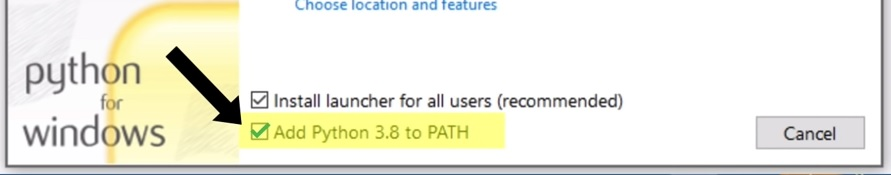
\includegraphics[width=0.65\textwidth]{python_path.jpg}
\end{alertblock}

\end{frame}

\begin{frame}
\begin{block}{Cross-Check}
\vspace{2pt}
Gib \bash{python} (Win) oder \bash{python3} (Mac) im \textit{Terminal} ein.
Du solltest etwa folgendes sehen:  
\vspace{12pt}

\texttt{Python 3.9.2 (tags/v3.9.2:1a79785, Feb 19 2021, 13:44:55) [MSC v.1928 64 bit (AMD64)] on win32
	Type "help", "copyright", "credits"{} or "license"{} for more information.}

\texttt{>{}>{}>}
\end{block}
\begin{block}{}
Jetzt bist Du im \textit{interactive mode} (REPL) von Python. Hier kannst Du einzelne Codezeilen eingeben und mittels \bash{Enter} ausführen. 
Um den interactive mode zu verlassen, gib \py{exit()} ein und bestätige mit der \bash{Enter}-Taste. 	
\end{block}
\end{frame}


%\begin{standout}
%	Erste Schritte im Interactive Mode\\
%\end{standout}
\section{Erste Schritte im REPL \\ \footnotesize (Read-Evaluate-Print-Loop)}


\begin{frame}
\begin{block}{Probier mal folgende Kommandos aus}	
	\begin{itemize}
		\item \py{3 + 4}
		\item \py{2 - 7}
		\item \py{"Hello" + "Python"}
	\end{itemize}
\end{block}	
\end{frame}



\begin{frame}{Übung}
\uncover<+->{\begin{block}{Was machen die folgenden \textit{Operatoren}?}
	\begin{itemize}
		\item \pybw{+}
		\item \pybw{-}
		\item \pybw{*}
		\item \pybw{/}
		\item \pybw{**}
	\end{itemize}
\end{block}}
\uncover<+->{\begin{block}{Und diese?}
\begin{itemize}
		\item \%
		\item \pybw{//}
		\item \pybw{==}
		\item \pybw{<=}
		\item \pybw{<}
\end{itemize}
\end{block}}

\end{frame}

\begin{frame}{Übung}
	\begin{block}{Wie rechnet Python?}
		\begin{itemize}
			\item Wird Punkt-vor-Strich berücksichtigt?
			\item Kann man mit Klammern die Reihenfolge beeinflussen?
			\item Was ist der Unterschied zwischen \py{10/5} und \py{10//5} ?
			\item Was bedeutet das Kommando \py{_}? 
			\item Wie kann man Zwischenergebnisse in Variablen speichern?
		\end{itemize}
	\end{block}
\end{frame}

\section{Variablen}

\begin{frame}
\uncover<+->{\begin{block}{}
		Jeder Wert in Python kann in einer Variable gespeichert werden: 
		
		\py{my_variable = 3}
\end{block}}

\uncover<+->{\begin{block}{}
		Die Zuweisung darf auch das Ergebnis einer Berechnung sein: 
		
		\py{my_new_variable = 3 + 5}
\end{block}}
\uncover<+->{\begin{block}{}
		Die Zuweisung darf auch weitere Variablen enthalten: 
		
		\py{my_brand_new_variable = my_variable + my_new_variable }
\end{block}}

\uncover<+->{\begin{block}{}
	Man darf auch Kettenzuweisungen machen: 
	
	\py{a = b = c = 100 }
\end{block}}
\end{frame}


\begin{frame}
\uncover<+->{\begin{block}{Gültige Variablennamen}
\begin{itemize}[<+->]
	\item Erlaubt sind Buchstaben (nur ASCII), Ziffern und Unterstriche
	\item Der Name darf nicht mit einer Ziffer starten
	\item Beliebige Länge 
	\item Wer's schon kennt als \emph{regulärer Ausdruck}:  \mintinline{php}{[_a-zA-Z][_0-9a-zA-Z]*}
	\item Schlüsselwörter sind nicht erlaubt
\end{itemize} 
\end{block}}
\vspace{12pt}
\uncover<+->{\begin{block}{Liste der Schlüsselwörter}
	\texttt{
	\begin{columns}[T,onlytextwidth]
		\column{0.2\textwidth}
		False\\ 	await\\ 	else\\ 	import\\ 	pass\\ assert \\	del\\ 	
		\column{0.2\textwidth}
		None \\	break \\	except \\ 	in \\	raise \\ global \\	not \\	 
		\column{0.2\textwidth}
		True \\	class \\ 	finally \\ 	is \\	return \\ with \\ async 
		\column{0.2\textwidth}
		and \\	continue \\ 	for \\	lambda \\	try \\ 	elif  \\	if  \\
		\column{0.2\textwidth}
		as \\ 	def \\ 	from  \\	nonlocal \\	while \\ 	or \\ 	yield
	\end{columns}
}
\end{block}}
\end{frame}


\begin{frame}
\uncover<+->{\begin{exampleblock}{Style-Guide Variablennamen}
	\begin{itemize}
		\item Englische Wörter
		\item Nur Kleinbuchstaben
		\item Möglichst aussdrucksstarke Namen verwenden
		\item Keine Angst vor langen Namen 
		\item Namen, die aus mehreren Worten bestehen, mit Unterstrich trennen (\textit{snake-case})
	\end{itemize}
	
	\uncover<+->{z.B. \py{students_in_this_room}, \py{number_of_unpaid_bills}}
\end{exampleblock}}

\end{frame}

\begin{frame}{Übung}
	
	\begin{block}{Probier's aus!}
		\begin{itemize}
			\item Welchen Wert hat eine Variable, wenn man sie nicht vorher definiert hat? 
			\item Was passiert, wenn man eine Variable definiert, die schonmal verwendet wurde?
			\item Wie kann man eine Variable mit Wert \py{3} um \py{1} vergrößern?
		\end{itemize}	
	\end{block}
	
\end{frame}


\section{Datentypen}

\begin{frame}
	\begin{block}{}
		Jeder Wert in Python hat einen \textit{Datentyp}. Unter anderem gibt es folgende \textit{primitive} Typen in Python.
		\begin{itemize}
			\item \py{int}  Integer (ganze Zahlen)
			\item \py{float} Float (Dezimalzahlen)
			\item \py{bool} Boolean (Wahrheitswerte)
			\item \py{str}  String (Zeichenketten)
			\item \pybw{NoneType} (Typ des leeren Werts \py{None})
		\end{itemize}
	\end{block}
\end{frame}


\begin{frame}
	\metroset{block=fill}
	
	\uncover<+->{\begin{block}{Integer}
		Ganze Zahlen wie z.B. \py{1}, \py{-1}, \py{0}. Nicht aber 
		\py{2.0} oder \py{0.0}. 	
	\end{block}}
	\vspace{12pt}
	\uncover<+->{\begin{block}{Float}
		Fließkommazahlen, z.B. \py{3.1415925}. Achtung: Bei Float-Berechnungen können schnell \enquote{Überraschungen} auftreten: Was ergibt z.B. \mintinline{python}{1.2 - 1.0} ? 
	\end{block}}
	\vspace{12pt}
	\uncover<+->{\begin{block}{Boolean}
		Booleans sind eine Sonderform von \py{int} und können nur die Werte \py{True} (entspricht 1) und \py{False} (entspricht 0) annehmen. Sie entstehen in der Regel, wenn man Fragen im Programm stellt (z.B. \py{3 < 4} oder \py{1 == 2}).   	
	\end{block}}
\end{frame}



\begin{frame}
	\metroset{block=fill}
	\uncover<+->{\begin{block}{String}
		Strings sind beliebige Zeichenketten und müssen in (ein-, zwei- oder dreifache) Anführungszeichen eingeschlossen werden. Die Ausdrücke \py{'hello'}, \py{"Hello"} und \py{"""Hello"""} sind (fast) äquivalent. 
	\end{block}}
	\vspace{12pt}

	\uncover<+->{\begin{block}{Mehrzeilige Strings}
		Ein \textit{Stringliteral} kann nur innerhalb einer Zeile definiert werden. Soll ein String mehrere Zeilen umfassen, müssen dreifache Anführungszeichen verwendet werden.  
	\end{block}}

	\end{frame}

	\begin{frame}
			\metroset{block=fill}
		\uncover<+->{\begin{block}{Steuerzeichen}
			Gewisse Kombinationen mit Backslash sind reservierte Steuerzeichen. So bezeichnet beispielsweise \py{\n} einen Zeilenumbruch und \py{\t} ein Tabulatorzeichen. \\
			Beispiel: \py{"This text\nfills two lines"}
		\end{block}}
			\vspace{12pt}
		\uncover<+->{\begin{block}{Escaping}
			Möchte man ein Steuerzeichen nicht ausführen, sondern buchstäblich nehmen. Muss man sie mit einem Backslash \textit{escapen} bzw. maskieren. \\
			Beispiel: \py{"This text fits in\\n one line"}
		\end{block}}
		\vspace{12pt}
		\uncover<+->{\begin{block}{Raw-Strings}
				Möchte man alle Steuerzeichen eines Strings ignorieren, kann man ihn als \textit{Raw-String} definieren. \\
				Beispiel: \py{r"This \n String \t has no control characters"}
		\end{block}}
		
	\end{frame}

	
	\begin{frame}
		\metroset{block=fill}
		\uncover<+->{\begin{block}{Typ einer Variablen ermitteln}
			\vspace{2pt}
			Mit der Funktion \py{type()} lässt sich der Typ bestimmen, z.B. \py{type(3.2)}.  	
		\end{block}}
		\vspace{12pt}
		\uncover<+->{\begin{block}{Typumwandlung (\emph{Typecasting})}
			\vspace{2pt}
			\uncover<+->{\textbf{Implizit}\\
			Bei manchen Operationen nimmt Python automatisch eine Typumwandlung vor. \\ Beispiel: \py{1 + 2.0} ergibt \py{3.0}	
		} \\ \\
		\uncover<+->{\textbf{Explizit \\}
			Die Funktionen \py{int()}, \py{float()}, \py{str()} und \py{bool()} führen jeweils eine Typumwandlung durch (sofern möglich). Beispiele: 
			\begin{itemize}
				\item \py{int(2.0)} ergibt \py{2} 
				\item \py{float(2)} ergibt \py{2.0} 
				\item \py{int("3")} ergibt \py{3}
			\end{itemize} 
		}
		\end{block}}
		
		
	\end{frame}
	
	
	\begin{frame}{Übung}
		
		\begin{block}{Versuche die Fragen erst ohne Python zu beantworten, überprüfe Deine Vermutung}
			\begin{itemize}
				\item Welchen Datentyp hat das Ergebnis von \py{3 - 1.0} ?
				\item Was ist das Ergebnis von \py{"2" + 1} ? 
				\item Was ist das Ergebnis von \py{"2"} + \py{"2"}? 
				\item Sind die beiden Werte \py{0} und \py{"0"} gleich? 
				\item Sind die beiden Werte \py{2} und \py{True} gleich? 
				\item Sind die beiden Werte \py{bool(2)} und \py{True} gleich? 
				\item Sind die beiden Werte \py{1} und \py{True} gleich? 
			\end{itemize}
		\end{block}
		
		
	\end{frame}

	\begin{frame}{Übung}
	
	\begin{block}{Erkläre mit Deinen eigenen Worten}
		\begin{itemize}
			\item Nach welcher Regel wandelt \py{int()} eine Fließkommazahl in eine ganze Zahl um? 
			\item Nach welchen Regeln wandelt \py{bool()} Zahlen und Strings in einen Wahrheitswert um? 
		\end{itemize}
	\end{block}
	
	
\end{frame}




\section{Operatoren}

\begin{frame}
\begin{block}{Die wichtigsten Operatoren}
	\begin{itemize}
		\item \pybw{+} (Addition oder Zusammenkleben von Strings)
		\item \pybw{-} (Subtraktion)
		\item \pybw{*} (Multiplikation)
		\item \pybw{/} (Division, ergibt immer ein Wert vom Typ \pybw{float})
		\item \pybw{**} (Potenzierung)
			\item \% (\textit{modulo-Operator}: Rest bei ganzzahliger Division)
		\item \pybw{//} (Division und Abrunden, ergibt immer ein Wert vom Typ \pybw{int})
		\item \pybw{==} (Vergleichsoperator, ergibt immer ein Wert vom Typ \pybw{bool})
		\item \pybw{!=} (Ungleichheitsoperator, ergibt das Gegenteil von \pybw{==})
	\end{itemize}
\end{block}
\end{frame}

\begin{frame}
\begin{block}{Operator-Präzedenz}
	\uncover<+->{
	\begin{enumerate}[<+->]
		\item Klammern
		\item \pybw{**}
		\item \pybw{*}, \pybw{/}, \pybw{//}, \%
		\item \pybw{+},\pybw{-}
	\end{enumerate}	
	}
\uncover<+->{
Operatoren gleichen Rangs werden innerhalb eines Ausdrucks von links nach rechts abgearbeitet. 
}

\uncover<+->{
\vspace{10pt}
\textbf{Ausnahmen:}\\
Potenzierung (\py{**}) und Zuweisung (\py{=}) werden von rechts nach links verarbeitet. 
}
\end{block}
\end{frame}

\begin{fragile}[]
\begin{block}{Kombinierte Zuweisung}
		\vspace{2pt}
		Oft möchte man eine gegebene Variable neu zuweisen: 
		\begin{minted}{python}
		counter = 1
		counter = counter + 1 	# counter = 2
		\end{minted}
		\pause
		Dies lässt sich auch kurz schreiben als 
		\begin{minted}{python}
		counter = 1
		counter += 1 	# counter = 2
		\end{minted}
		\pause
		Analog sind die Operatoren \py{-=}, \py{*=}, \py{/=}, etc. definiert. 
	\end{block}
\end{fragile}



\section{Input/Output \\ \footnotesize Teil 1}

\begin{fragile}[]

\begin{block}{Output}
	\vspace{2pt}
	Um einen String auf der \emph{Konsole} auszugeben, verwende die Funktion \py{print()}. 
	
	
	Zum Beispiel \py{print("Hello there")}. 
	\pause
	
	Es können auch Variablen eingesetzt werden: 
	\begin{minted}{python}
	message = "Hello there"
	print(message) # Hello there
	\end{minted}
	
	\end{block}
	
\end{fragile}

\begin{fragile}[]
	
\begin{block}{String Interpolation}
\vspace{2pt}
Um Variablenwerte innerhalb eines Strings auszugeben, verwenden wir die String-Interpolation-Syntax:
\begin{minted}{python}
my_value = 5
print(f"The variable my_value has the value {my_value}")
# The variable my_value has the value 5
\end{minted}
\pause
Das geht auch als \textit{inline expression}: 
\begin{minted}{python}
print(f"The sum of 1 and 2 is {1+2}")
# The sum of 1 and 2 is 3
\end{minted}

\end{block}
	
\end{fragile}

\begin{fragile}
\begin{block}{Output}
	\vspace{2pt}
Um einen String vom User einzulesen, verwende die Funktion \py{input()}:

\begin{minted}{python}
age = input("How old are you?")
print(f"I am {age} years old")
\end{minted}
\end{block}
\pause 
\begin{alertblock}{Achtung}
	\vspace{2pt}
Das Ergebnis von \py{input} hat stets den Datentyp \py{string} auch wenn Zahlen eingelesen werden. Gegebenenfalls muss das Ergebnis mittels \py{int()} oder \py{float()} in den gewünschten Typ umgewandelt werden. 	
\end{alertblock}

\end{fragile}

\section{Script Mode}
\begin{frame}
\begin{block}{Script Mode}
	\vspace{2pt}
	Sobald man mehrere zusammenhängende Zeilen hat, wird Pythons \textit{interactive mode} sehr unübersichtlich. Daher gibt es auch die Möglichkeit, alle Programmzeilen in eine Text-Datei zu schreiben und diese gebündelt auszuführen.   
\end{block}

\end{frame}
\begin{fragile}[]
	\begin{exampleblock}{Ein erstes Beispiel}
		\begin{minted}{python}
		name = input("What is your name?")
		age = input("What is your age?")
		print(f"Hello {name}, you are {age} years old") 
		\end{minted}
		
		Speichere diesen Code in der Datei \pybw{my_script.py} ab. 
		
		Führe danach in diesem Ordner das Kommando 
		\pybw{python my_script.py} aus. 
	\end{exampleblock}
\end{fragile}

\begin{frame}{Übung}
	Schreibe ein kurzes Skript, dass Dich nach Deinem Namen, Alter und Adresse fragt. Wenn es alles eingelesen hat, soll es diese Infos in folgender Form auf der Konsole ausgeben: 	
	
	\texttt{Hallo Max, schön dass Du da bist. Du bist 21 Jahre alt und wohnst in der Bismarckstraße 12 in Glücksstadt.}
	
\end{frame}


\begin{fragile}
	
	\begin{block}{Kommentare}
		\vspace{2pt}
		Alle Zeichen einer Zeile, die hinter einem \texttt{\#} (Hashtag) kommen, werden von Python ignoriert.
		So lassen sich Kommentare im Quellcode platzieren. 
	\end{block}
	\vspace{12pt}
	\begin{exampleblock}{Beispiel}
	\begin{minted}{python}
	print("This line will be printed")
	# print("This line won't") 
	\end{minted}
	\end{exampleblock}
	
\end{fragile}


\section{Arbeit mit einer IDE}

\begin{frame}
	\begin{block}{Integrierte Entwicklungsumgebungen (IDE)}
		\vspace{2pt}
		\uncover<+->{
	Die Arbeit mit gewöhnlichen Texteditoren ist auf Dauer sehr mühsam. Daher empfiehlt es sich eine IDE zu verwenden. 
	Das bringt zum u.a. folgende Vorteile: 
	\begin{itemize}[<+->]
		\item Syntax-Highlighting
		\item Code-Inspection
		\item Autocomplete
		\item Geile Shortcuts
		\item Code direkt ausführen
		\item Hilfe bei der Fehlersuche (\emph{Debugging})
	\end{itemize}	
		}
	\end{block}
\end{frame}

\begin{frame}
	\uncover<+->{
	\begin{block}{Installation von PyCharm}
		\vspace{2pt}
		\begin{enumerate}
			\item Gehe auf 
			\texttt{https://www.jetbrains.com/pycharm/download} \\
			\item Lade die kostenlose \textit{Community Edition} herunter
			\item Führe den Installer aus
			\item Öffne PyCharm
		\end{enumerate}
	\end{block}
	}
	
\uncover<+->{
	\begin{block}{Wenn alles passt, sollte es etwa so aussehen:}
		\vspace{2pt}
		\begin{center}
		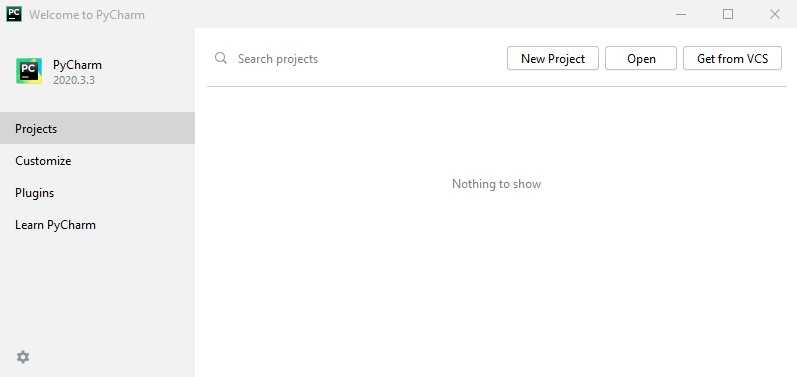
\includegraphics[width=0.65\textwidth]{pycharme.jpg}
		\end{center}
	\end{block}
}	
	
\end{frame}



\begin{frame}
	\begin{block}{Installation PyCharm}
		\vspace{2pt}
		\begin{enumerate}
			\item Gehe auf \texttt{Customize > All Settings...}
			\item Einstellungen synchronisieren
			\begin{enumerate}
				\item \texttt{Tools > Settings Repository}
				\item Unter \textit{Read-only Sources} auf \texttt{+}
				\item \texttt{https://github.com/a-kunert/ide-settings.git}	eingeben
				%\item  File > Manage IDE Settings > Sync with Settings Repository > Merge ausführen 
			\end{enumerate}
			\item Verknüpfe den Interpreter
			\begin{enumerate}
				\item In den Settings auf \texttt{Python Interpreter}
				\item Falls möglich unter \texttt{Python Interpreter} einen Interpreter wählen. Ansonsten wie folgt: 
				\item \texttt{Zahnrad > Add}
				\item \texttt{System Interpreter}
				\item Dort den Pfad zu Python angeben
			\end{enumerate}
			\item Mit dem Button \textit{Apply} alles bestätigen
		\end{enumerate}
	\end{block}
\end{frame}

\begin{frame}
	\begin{block}{Konfiguration abschließen}
		\begin{enumerate}
		\item Lege eine Ordner für den Kurs an
		\item Öffne diesen Ordner mit \texttt{Projects > Open}
		\item \texttt{File > Manage IDE Settings > Sync with Settings Repository > Merge} ausführen
		\item Bei \texttt{File > Settings} unter \texttt{Keymap} die Keymap \textit{Salem-Win/Mac} auswählen. 
		\item Code in die Datei \texttt{main.py} schreiben
		\item Mittels grünem Pfeil (oben rechts) Code ausführen
	\end{enumerate}	
	\end{block}
\end{frame}


\section{Script Mode}
\begin{frame}
\begin{block}{Script Mode}
	\vspace{2pt}
	Sobald man mehrere zusammenhängende Zeilen hat, wird die REPL sehr unübersichtlich. Daher gibt es auch die Möglichkeit, alle Programmzeilen zunächst aufzuschreiben und diese dann gebündelt von Python ausführen zu lassen. Im Gegensatz zum REPL bzw. interactive Mode von Python wird dies \emph{Script Mode} genannt.    
\end{block}
\end{frame}

\begin{fragile}[]
\begin{exampleblock}{Beispiel}
\begin{minted}{python}
name = "Max"
age = 20
print(f"Hello, I'm {name} and I'm {age} years old") 
\end{minted}
\end{exampleblock}
\pause
\begin{alertblock}{Problem:}
\vspace{2pt}
Wie kann man Python erklären, diese 3 Zeilen auf einmal auszuführen? 
\end{alertblock}
\end{fragile}

\begin{frame}
\begin{block}{Old-School-Lösung}
\vspace{2pt}
\begin{itemize}
	\item Erstelle eine neue Datei (z.B. \pybw{my_script.py})
	\item Öffne die Datei mit einem Texteditor und speichere den Beispiel-Code darin ab.
	\item Öffne den Ordner mit der Datei \pybw{my_script.by} mit dem Terminal bzw. der Eingabeaufforderung
	\item Führe das Kommando \pybw{python my_script.py} aus. 
\end{itemize}
\end{block}
\end{frame}

\begin{frame}
\begin{block}{Optimallösung: Verwende eine IDE}
	\vspace{2pt}	
	Eine IDE (integrierte Entwicklungsumgebung) hilft Dir beim Programmieren und unterstüzt Dich wo immer möglich. Dadurch lassen sich auch große Projekte schnell umsetzen. 
\end{block}
\begin{alertblock}{Nachteile}
	\vspace{2pt}
	Die anfängliche Einrichtung kann schnell mal kompliziert werden. Aufgrund der vielen Features fühlt man sich schnell mal überfordert. 
	
	$\rightarrow$ Das kommt erst später.	
\end{alertblock}
\end{frame}


\begin{frame}
\begin{block}{Kompromiss für den Anfang: Browserbasierte Editoren}
\vspace{2pt}
Um schnell einzusteigen, kann zu Beginn auch ein browsergestützter Editor/Interpreter verwendet werden. Zum Beispiel: 
\pause
\begin{itemize}
	\item Programiz (\texttt{https://www.programiz.com/python-programming/online-compiler})
	\begin{itemize}
		\item einfacher Einstieg
		\item schnell und unkompliziert
		\item geringer Funktionsumfang
	\end{itemize}
	\pause
	\item Repl.it (\texttt{https://replit.com/languages/python3})
	\begin{itemize}
		\item Auch für viele andere Sprachen geeignet
		\item Manchmal etwas langsam
		\item Man kann mehrere Dateien und Projekte verwalten (braucht Account) 
		\item Hat fast alle IDE-Features (braucht Account)
	\end{itemize}
%	\item Onecompiler (\texttt{https://onecompiler.com/python})
%	\begin{itemize}
%		\item Benötigt immer einen Account
%		\item Viele Funktionen
%	\end{itemize}
\end{itemize}
\end{block}

\end{frame}



\section{Input/Output \\ \footnotesize Teil 1}


\begin{frame}

\begin{block}{Die Konsole}
\vspace{2pt}
Da wir zu Beginn noch über keine grafische Benutzeroberfläche verfügen, verwenden wir für die Kommunikation mit unserem Programm die \emph{Konsole}. 
Dabei handelt es sich um ein einfaches Textfenster, auf dem Dein Programm Informationen ausgeben kann (\emph{Output}) und Text einlesen kann (\emph{Input}). 
\end{block}

\end{frame}

\begin{fragile}[]
	
	\begin{block}{Output}
		\vspace{2pt}
		Um einen String auf der \emph{Konsole} auszugeben, verwende die Funktion \py{print()}. 
		
		
		Zum Beispiel \py{print("Hello there")}. 
		\pause
		
		Es können auch Variablen eingesetzt werden: 
		\begin{minted}{python}
		message = "Hello there"
		print(message) # Hello there
		\end{minted}
		
	\end{block}
	
\end{fragile}

\begin{fragile}[]
	
	\begin{block}{String Interpolation}
		\vspace{2pt}
		Um Variablenwerte innerhalb eines Strings auszugeben, verwenden wir die String-Interpolation-Syntax:
		\begin{minted}{python}
		my_value = 5
		print(f"The variable my_value has the value {my_value}")
		# The variable my_value has the value 5
		\end{minted}
		\pause
		Das geht auch als \textit{inline expression}: 
		\begin{minted}{python}
		print(f"The sum of 1 and 2 is {1+2}")
		# The sum of 1 and 2 is 3
		\end{minted}
		
	\end{block}
	
\end{fragile}

\begin{fragile}
	\begin{block}{Input}
		\vspace{2pt}
		Um einen String vom User einzulesen, verwende die Funktion \py{input()}:
		
		\begin{minted}{python}
		age = input("How old are you?")
		print(f"I am {age} years old")
		\end{minted}
	\end{block}
	\pause 
	\begin{alertblock}{Achtung}
		\vspace{2pt}
		Das Ergebnis von \py{input} hat stets den Datentyp \py{string} auch wenn Zahlen eingelesen werden. Gegebenenfalls muss das Ergebnis mittels \py{int()} oder \py{float()} in den gewünschten Typ umgewandelt werden. 	
	\end{alertblock}
	
\end{fragile}


\begin{fragile}[]
	\begin{exampleblock}{Beispiel: Input und Output kombiniert}
		\begin{minted}{python}
		name = input("What is your name?")
		age = input("What is your age?")
		print(f"Hello {name}, you are {age} years old") 
		\end{minted}
	\end{exampleblock}
\end{fragile}

\begin{frame}{Übung}
Schreibe ein kurzes Skript, dass Dich nach Deinem Namen, Alter und Adresse fragt. Wenn es alles eingelesen hat, soll es diese Infos in folgender Form auf der Konsole ausgeben: 	

\texttt{Hallo Max, schön dass Du da bist. Du bist 21 Jahre alt und wohnst in der Bismarckstraße 12 in Glücksstadt.}
\end{frame}


\begin{frame}{Übung}
Schreibe ein kurzes Skript, dass Dich nach Deinem Alter fragt. Daraufhin soll es auf der Konsole ausgeben, wie alt Du in 15 Jahren sein wirst. 
\end{frame}


\begin{fragile}

\begin{block}{Kommentare}
\vspace{2pt}
Alle Zeichen einer Zeile, die hinter einem \texttt{\#} (Hashtag) kommen, werden von Python ignoriert.
So lassen sich Kommentare im Quellcode platzieren. 
\end{block}
\vspace{12pt}
\begin{exampleblock}{Beispiel}
\begin{minted}{python}
print("This line will be printed")
# print("This line won't") 
\end{minted}
\end{exampleblock}

\end{fragile}



\section{Conditionals \\ \footnotesize Ein Programm verzweigen}

\begin{frame}
	\begin{block}{Problemstellung}
		\vspace{2pt}
		Lies eine Zahl \py{x} ein. In Abhängigkeit von \py{x} soll Folgendes ausgegeben werden: 
		
		\texttt{Die Zahl x ist größer als 0} 
		
		bzw. 
		
		\texttt{Die Zahl x ist kleiner 0}  
		\vspace{8pt}
		
		Wie macht man das?
		\end{block}
\end{frame}

\begin{fragile}
	
\begin{block}{Lösung \footnotesize(fast)}
\begin{minted}{python}
x = int(input("Gib eine Zahl x an"))

if x < 0:
  print("x ist größer 0")
else:
  print("x ist kleiner 0")
\end{minted}
\end{block}
	
\end{fragile}


\begin{frame}
\metroset{block=fill}


	\renewcommand{\baselinestretch}{1.5}
\begin{block}{Struktur \texttt{if-else} Statement}	
	\vspace{2pt}
	\uncover<+->{
	\uncover<+->{\texttt{if}} \uncover<+->{\textit{Bedingung}}\uncover<+->{\texttt{:}}\\
	\uncover<+->{\spacechar\spacechar }\uncover<+->{\textit{Codezeile A1}}	\\
	\uncover<+->{\spacechar\spacechar \textit{Codezeile A2}	\\
	\spacechar\spacechar \phantom{Code}\vdots}\\
	\uncover<+->{\texttt{else:}}\\
	\uncover<+->{\spacechar\spacechar \textit{Codezeile B1}	\\
				 \spacechar\spacechar \textit{Codezeile B2}	\\
				 \spacechar\spacechar \phantom{Code}\vdots}\\
	\uncover<+->{\textit{Codezeile C1}\\
	\phantom{Code}\vdots
}
}
\end{block}
\renewcommand{\baselinestretch}{1}
%\vspace{10pt}

\end{frame}
\begin{frame}
\begin{block}{Wie funktioniert's?}
	\vspace{2pt}
Ist die \texttt{if}-Bedingung \py{True}, so wird der \texttt{if}-\textit{Block} ausgeführt. Ist sie \py{False} wird der \texttt{else}-\textit{Block} ausgeführt 
\end{block}
\pause

\vspace{10pt}
\metroset{block=fill}
	\begin{block}{Definition Block}
		\vspace{2pt}
		Aufeinanderfolgende Codezeilen, die alle die gleiche Einrückung besitzen, nennt man \emph{Block}. 
		D.h. Leerzeichen am Zeilenanfang haben in Python eine syntaktische Bedeutung.  
	\end{block}


\pause 
\vspace{10pt}

\metroset{block=transparent}
\begin{block}{Good to know}
	\begin{itemize}
		\item Der \pybw{else}-Block ist optional.
		\item Falls die Bedingung nicht vom Typ \py{bool} ist, so wird sie implizit umgewandelt.  
	\end{itemize}
\end{block}
\end{frame}

\begin{frame}{Übungen}

	\begin{block}{Volljährigkeit prüfen/Zutrittskontrolle}
		\vspace{2pt}
		Schreibe ein Skript, dass nach dem Alter eines Users fragt und überprüft, ob der User schon volljährig ist. Dementsprechend soll auf der Konsole entweder 
		
		\texttt{Willkommen}
		
		 oder
		 
		  \texttt{Du darfst hier nicht rein} 
		  
		  erscheinen.  
	\end{block}
\pause 
\vspace{12pt}
	\begin{block}{Teilbarkeit bestimmen}
		\vspace{2pt}
		Schreibe ein Skript, dass eine ganze Zahl einliest. Daraufhin soll auf der Konsole ausgegeben werden, ob die Zahl durch \pybw{7} teilbar ist. Beispiel: Ist die Eingabe 12, so ist die Ausgabe:   

		\texttt{Die Zahl 12 ist nicht durch 7 teilbar.}
	\end{block}

\end{frame}



\begin{frame}

\metroset{block=fill}
\uncover<+->{\begin{block}{Logische Operatoren}
	\vspace{2pt}
Booleans können mittels folgender Operatoren miteinander verknüpft werden
\begin{description}
	\item[\pybw{and}] Ist genau dann \py{True}, wenn beide Operanden \py{True} sind.
	\item[\pybw{or}] Ist genau dann \py{True}, wenn mindestens ein Operand \py{True} ist.
	\item[\pybw{not}] Kehrt den nachfolgenden Wahrheitswert um.  
\end{description}
\end{block}}
\vspace{10pt}
\metroset{block=transparent}
\uncover<+->{\begin{exampleblock}{Beispiel}
\begin{itemize}
	\item \pybw{2 > 0 and 3 > 4} ist \py{False}
	\item \pybw{1 > 0 or 6 > 1} ist \py{True}
	\item \pybw{not 2 < 1} ist \py{True}
\end{itemize}
\end{exampleblock}
}
\end{frame}


\begin{frame}{Übung}
\uncover<+->{
\begin{block}{Was ergeben die folgenden Ausdrücke?}
	\begin{itemize}
		\item \py{not 2 < 3 and 4 < 7}
		\item \py{4 not == 8}
		\item \py{3 != 4 and not 4 == 8}
		\item \py{7 <= 7.0 and not 7 != 7.0}
		\item \py{7 > 5 or 4 < 5 and not 9 > 6}
		\item \py{not 3 < 6 > 8}
		\item \py{not 3}
	\end{itemize}
\end{block}
}
\uncover<+->{
\begin{alertblock}{Präzedenz beachten!}
	\begin{enumerate}
		\item \pybw{==}, \pybw{!=}, \pybw{<=}, \pybw{<}, \pybw{>}, \pybw{>=}
		\item \pybw{not}
		\item \pybw{and}
		\item \pybw{or}
	\end{enumerate}
\end{alertblock}
}

\end{frame}

\begin{fragile}

\begin{block}{Das \pybw{elif}-Statement}
	\vspace{2pt}
Mit der reinen \pybw{if-else}-Syntax können nur \emph{binäre} Verzweigungen dargestellt werden. Um mehrer, gleichrangige Verzweigungsäste zu realisieren kann man das \pybw{elif}-Conditional verwenden. 
\end{block}
\pause
\begin{exampleblock}{Beispiel}
\begin{minted}{python}
if x < 0: 
    print("x is < 0")
elif x == 0: 
    print("x is 0")
elif x == 1: 
    print("x is 1")
else: 
    print("x is not negative but neither 0 nor 1")         
\end{minted}
\end{exampleblock}
\pause
Die Anzahl der \pybw{elif}-Blöcke ist beliebig. Der \pybw{else}-Block ist wie immer optional. 

\end{fragile}

\begin{fragile}{Übung}
	\begin{block}{Für welche \pybw{x} unterscheiden sich die beiden Abschnitte?}
		\vspace{5pt}
		Abschnitt 1: 
		\begin{minted}{python}
		if x % 2 == 0: 
		   # some Code here
		if x % 3 == 0: 
		   # some Code here
		else: 
		   # some Code here  
		\end{minted}
		Abschnitt 2: 
		\begin{minted}{python}
		if x % 2 == 0: 
		# some Code here
		elif x % 3 == 0: 
		# some Code here
		else: 
		# some Code here  
		\end{minted}
	\end{block}
\end{fragile}

\begin{frame}{Übung}
\begin{block}{Baue einen Bestätigungsdialog}
\vspace{2pt}
Schreibe ein Skript was einen typischen Bestätigungsdialog simuliert. 
Zum Beispiel: \texttt{Are you sure to continue? (y)es/(n)o}. Mögliche Antworten sind \texttt{yes}, \texttt{no} bzw. \texttt{y}, \texttt{n}. 
Daraufhin soll auf der Konsole \texttt{continued} oder \texttt{aborted} erscheinen. 
\end{block}
\end{frame}

\begin{frame}{Komplexere Übung}
%\begin{block}{Berechne Deinen Urlaubsort}
%\vspace{2pt}
%\end{block}
\begin{center}

\includegraphics[width=0.5\textwidth]{urlaubsort.png}
\end{center}
Lies eine Zahl zwischen 1 und 9 ein und gib auf der Konsole \emph{deinen nächsten Urlaubsort} aus. 
\end{frame}


\begin{fragile}{}
\begin{block}{Der \emph{Ternary Operator}}
\vspace{2pt}
Oftmals möchte man eine Variable in Abhängigkeit eines Wahrheitswertes definieren. Für diesen einfachen Fall, ist das \pybw{if-else}-Konstrukt sehr umständlich. Stattdessen kann man für die Kürze den \emph{ternary operator} verwenden. 
\end{block}
\vspace{12pt}
\pause
\begin{exampleblock}{Beispiel}
	\vspace{2pt}
	\begin{minted}{python}
	if x < 0: 
	  sign = "sign"	
	else: 
	  sign = "positive"
	\end{minted}
\end{exampleblock}
\pause 
\begin{block}{Stattdessen mit Ternary Operator}
	\vspace{2pt}
	\py{sign = "negative" if x < 0 else "positive"}
\end{block}
\end{fragile}

\begin{frame}{Übung}

\begin{block}{}
	\vspace{2pt}
Lies eine ganze Zahl ein und gib ihren Betrag auf der Konsole aus. Schaffst Du es, das Ganze mit weniger als 5 Zeilen Code zu programmieren? 
\end{block}

\end{frame}

\section{Die For-Schleife \\ \footnotesize Einen Programmabschnitt x-mal ausführen}

\begin{frame}

\begin{block}{Problemstellung}
\vspace{2pt}
Lies eine ganze Zahl \py{x} ein. Gib dann folgende Zeilen auf der Konsole aus 

\texttt{1}\\
\texttt{2}\\
\texttt{3}\\
\texttt{4}\\
\vdots \\
\texttt{x}

\vspace{12pt}
Wie macht man das? 

\end{block}
\end{frame}

\begin{fragile}{}
	\begin{block}{Lösung}
		\begin{minted}{python}
			x = input("Enter a number")
			
			for k in range(1, x + 1):	
			  print(k)
		\end{minted}
	\end{block}
\end{fragile}

\begin{frame}

	\renewcommand{\baselinestretch}{1.5}
	\metroset{block=fill}
	\begin{block}{Struktur der \texttt{for...in} Schleife}
		\vspace{2pt}
		\pause \py{for} \pause \textit{Variable} \pause \py{in} \pause \py{range}(\textit{min}, \textit{max})\pause\texttt{:} \pause \\
		\spacechar\spacechar Codezeile 1 \pause \\ 
\spacechar\spacechar Codezeile 2 \pause \\
\spacechar\spacechar \phantom{Code} \vdots \pause  \\
\textit{Code, der nicht mehr Teil der Schleife ist}
	\end{block}

\vspace{12pt}
\pause 

\metroset{block=transparent}
	\renewcommand{\baselinestretch}{1}
	\begin{block}{Wie funktioniert's?}
		\vspace{2pt}
	Die Schleifenvariable wird zunächst gleich dem unteren Wert in \py{range} gesetzt. Dann wird der \pybw{for}-Block wiederholt ausgeführt. Bei jedem Durchgang wird die Schleifenvariable um \pybw{1} vergrößert und zwar so lange, wie der Wert der Schleifenvariable kleiner als der obere Wert in \py{range} ist. 	
	\end{block}
\end{frame}

\begin{frame}
\begin{block}{Good to know}
	\pause
	\begin{itemize}[<+->]
		\item Achtung: Die Schleifenvariable erreicht nie das obere Ende der \py{range}-Funktion, sondern bleibt immer \pybw{1} drunter. 
		\item Die \py{range}-Funktion ist nicht auf 1er-Schrittweite beschränkt. Mit folgendem Ausdruck werden die Zahlen von \py{0} bis \py{9} z.B. in 3er-Schritten durchlaufen: \py{range(0, 10, 3)}. 
		\item \texttt{For}-Schleifen sind flexibel und können alles mögliche durchlaufen, z.B. auch die einzelnen Buchstaben eines Strings (dazu später mehr).
	\end{itemize}
\end{block}
\end{frame}

\begin{frame}{Übung}

\begin{block}{Einmaleins: Die 7er-Reihe}
	\vspace{2pt}
Schreibe ein kleines Skript, was die 7er-Reihe (bis 70) auf der Konsole ausgibt.	
\end{block}

\vspace{12pt}

\pause 

\begin{block}{7er-Reihe mit beliebigem oberen Ende}
	\vspace{2pt}
	Lies eine positive ganze Zahl \py{x} ein, gib die 7er-Reihe von \py{7} bis \py{x} auf der Konsole aus.  
\end{block}

\vspace{12pt}

\pause 

\begin{block}{7er-Reihe mit ganzen Sätzen}
	\vspace{2pt}
Lies wie eben eine obere Grenze für die 7-er Reihe ein. Gib dann die 7-er Reihe wie folgt auf der Konsole aus:

\texttt{1 mal 7 ist 7}\\	
\texttt{2 mal 7 ist 14}\\
\phantom{4 mal} \vdots

\end{block}
\end{frame}


\begin{frame}{Schwierigere Übung}

\begin{block}{Das Gauss-Problem}
\vspace{2pt}	
Berechne die Summe der Zahlen 1 bis 100. 
\end{block}
\vspace{12pt}
\pause
\begin{block}{Zahlenmuster}
\vspace{2pt}	
Gib folgendes Muster auf der Konsole aus: 

\texttt{1} \\
\texttt{1 2} \\
\texttt{1 2 3} \\
\texttt{1 2 3 4} \\
\phantom{1 2 } \vdots \\
\texttt{1 2 $\cdots$ 20}
\end{block}

\end{frame}

\begin{frame}{Harte Übungen}

\begin{block}{Quersumme}
	\vspace{2pt}
	Lies eine ganze Zahl \py{x} ein und bestimme ihre Quersumme. 
	
	\textbf{Tipp 1:} Die Anzahl der Stellen einer Zahl bekommt man mittels \py{len(str(x))} heraus. \\
	\textbf{Tipp 2:} Man benötigt Tipp 1 gar nicht.  
	
\end{block}

\vspace{12pt}
\pause

\begin{block}{Primzahltest}
	\vspace{2pt}
	Lies eine ganze Zahl \py{x} ein und überprüfe, ob diese Zahl eine Primzahl ist. Das Programm soll etwa folgende Ausgabe liefern 
	
	\texttt{Die Zahl 28061983 ist eine Primzahl.}
\end{block}

\end{frame}


\section{Die While-Schleife \\ \footnotesize Wie die For-Schleife nur abstrakter und open-end}

\begin{frame}
\begin{block}{Problemstellung}
	\vspace{2pt}
	Lies immer wieder eine Zahl von der Konsole ein. Höre auf, wenn diese Zahl 7 ist. 
	
	Wie macht man das? 
\end{block}
\end{frame}

\begin{fragile}
	
\begin{block}{Lösung}
		\vspace{2pt}
		
	\begin{minted}{python}
		x = 0
		
		while x != 7: 
		  x = input("Enter a number")
		  x = int(x)
		  
		print("Yeah, you picked the right number.")
	\end{minted}
	
\end{block}
\end{fragile}

\begin{frame}

\renewcommand{\baselinestretch}{1.5}
\metroset{block=fill}
\begin{block}{Struktur der \texttt{While}-Schleife}
	\vspace{2pt}
	\pause \py{while} \pause \textit{Bedingung}\pause\texttt{:} \pause \\
	\spacechar\spacechar Codezeile 1 \pause \\ 
	\spacechar\spacechar Codezeile 2 \pause \\
	\spacechar\spacechar \phantom{Code} \vdots \pause  \\
	\textit{Code, der nicht mehr Teil der Schleife ist}
\end{block}
\vspace{12pt}
\pause 
\metroset{block=transparent}
\renewcommand{\baselinestretch}{1}
\begin{block}{Wie funktioniert's?}
	\vspace{2pt}
	Die Schleife wird solange ausgeführt, wie die \emph{Bedingung} \py{True} ergibt. Nach jedem Durchgang wird der Ausdruck der \emph{Bedingung} neu ausgewertet. 
	Ist die Bedingung \py{False} wird der Code unterhalb des Schleifenblocks ausgeführt. 
\end{block}



\end{frame}




\section{Arbeit mit einer IDE}

\begin{frame}
\begin{block}{Integrierte Entwicklungsumgebungen (IDE)}
	\vspace{2pt}
	\uncover<+->{
		Die Arbeit mit gewöhnlichen Texteditoren ist auf Dauer sehr mühsam. Daher empfiehlt es sich eine IDE zu verwenden. 
		Das bringt zum u.a. folgende Vorteile: 
		\begin{itemize}[<+->]
			\item Syntax-Highlighting
			\item Code-Inspection
			\item Autocomplete
			\item Geile Shortcuts
			\item Code direkt ausführen
			\item Hilfe bei der Fehlersuche (\emph{Debugging})
		\end{itemize}	
	}
\end{block}
\end{frame}

\begin{frame}
\uncover<+->{
\begin{block}{Installation von PyCharm}
	\vspace{2pt}
	\begin{enumerate}
		\item Gehe auf 
		\texttt{https://www.jetbrains.com/pycharm/download} \\
		\item Lade die kostenlose \textit{Community Edition} herunter
		\item Führe den Installer aus
		\item Öffne PyCharm
	\end{enumerate}
\end{block}
}

\uncover<+->{
\begin{block}{Wenn alles passt, sollte es etwa so aussehen:}
	\vspace{2pt}
	\begin{center}
		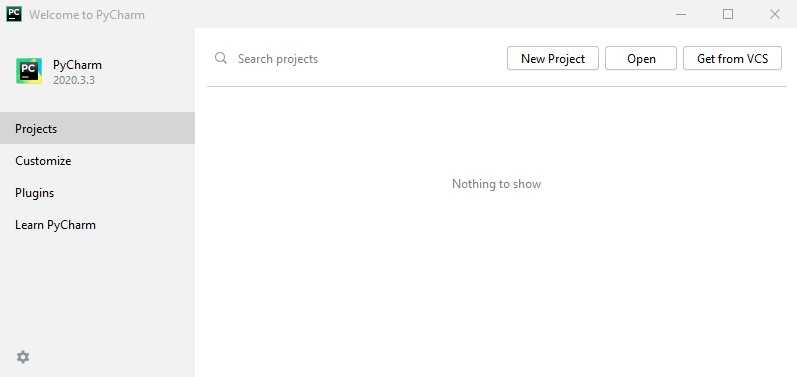
\includegraphics[width=0.65\textwidth]{pycharme.jpg}
	\end{center}
\end{block}
}	

\end{frame}








\begin{frame}
\begin{block}{Installation PyCharm}
\vspace{2pt}
\begin{enumerate}
\item Gehe auf \texttt{Customize > All Settings...}
\item Einstellungen synchronisieren
\begin{enumerate}
	\item \texttt{Tools > Settings Repository}
	\item Unter \textit{Read-only Sources} auf \texttt{+}
	\item \texttt{https://github.com/a-kunert/ide-settings.git}	eingeben
	%\item  File > Manage IDE Settings > Sync with Settings Repository > Merge ausführen 
\end{enumerate}
\item Verknüpfe den Interpreter
\begin{enumerate}
	\item In den Settings auf \texttt{Python Interpreter}
	\item Falls möglich unter \texttt{Python Interpreter} einen Interpreter wählen. Ansonsten wie folgt: 
	\item \texttt{Zahnrad > Add}
	\item \texttt{System Interpreter}
	\item Dort den Pfad zu Python angeben
\end{enumerate}
\item Mit dem Button \textit{Apply} alles bestätigen
\end{enumerate}
\end{block}
\end{frame}

\begin{frame}
\begin{block}{Konfiguration abschließen}
\begin{enumerate}
\item Lege eine Ordner für den Kurs an
\item Öffne diesen Ordner mit \texttt{Projects > Open}
\item \texttt{File > Manage IDE Settings > Sync with Settings Repository > Merge} ausführen
\item Bei \texttt{File > Settings} unter \texttt{Keymap} die Keymap \textit{Salem-Win/Mac} auswählen. 
\item Code in die Datei \texttt{main.py} schreiben
\item Mittels grünem Pfeil (oben rechts) Code ausführen
\end{enumerate}	
\end{block}
\end{frame}


\end{document}






